%%%%%%%%%%%%%%%%%%%%%%%%%%%%%%%%%%%%%%%%%%
\chapter{Modeling CFD-DEM} \label{modelingCFDEM}
%%%%%%%%%%%%%%%%%%%%%%%%%%%%%%%%%%%%%%%%%%
[talk about how lacking the DEM result is without the inclusion of helium in analysis. There are some Fusion papers on conductivity in vacuum and with helium]

We now consider the influence of helium on thermal transport of deposited nuclear energy as it is carried away by the cooled structural walls. We begin by considering the fluid in a continuum sense and the pebbles in a discrete one. The interactions of the fluid and solid are characterized by effective relationships in each discretized cell of fluid. We then consider an mesoscopic approach to the fluid-solid interaction with the Lattice-Boltzmann method. 

The chapter begins with introduction of the coupled fluid dynamics - discrete element method (CFD-DEM) approach: governing equations, discretization techniques, and algorithms.

We then do LBM. And stuff.

%%%%%%%%%%%%%%%%%%%%%%%%%%%%%%%%%%%%%%%%%%
\section{Numerical Methodology}
% From TOFE 2014
Models based on the discrete element method (DEM) are currently the only tools available that can extract information on individual pebble interactions. The DEM formulation provides information such as inter-particle forces and individual particle temperatures, which are necessary for predicting and simulating morphological changes in the bed (e.g. pebble cracking, sintering, etc.) However DEM alone is not able to capture the effects, neither on momentum nor energy, of an interstitial fluid. Therefore we present two fluid modeling techniques to supplement the DEM computations. We will first discuss the fully dynamic coupling of the DEM model with a volume-averaged thermofluid model of helium. Then we will introduce the integration of our DEM packing structure into lattice-Boltzmann simulations of the entire bed-fluid system.

\subsection{DEM}\label{sec:cfdem-heat-transfer}
The discrete element framework introduced in \S~\ref{sec:particle-dynamics} is augmented with a drag force term to capture interaction with surrounding fluid velocity fields. To accomplish this, we simply include a drag force to the Newtonian balance of forces given in Eq.~\ref{eq:newtons-first}. The momentum balance now reads:

\begin{equation}\label{eq:cfdem-dem-momentum}
	m_i  \ddt{\vec{r}_i} = m_i\vec{g} + \vec{f}_i + \beta_i V_i \Delta u_{if}
\end{equation}

where $\Delta u_{if} = u_f - u_i$, is the relative velocity between the fluid and pebble, $i$, and the inter-phase momentum exchange coefficient, $\beta_i$, acts upon the pebble volume (not to be confused with the damping coefficient introduced in \S~\ref{sec:particle-dynamics}). Similarly, the energy equation now includes 

\begin{equation}\label{eq:cfdem-dem}
	m_iC_i \ddt{T_i} = Q_{n,i} + \sum_{j=1}^Z Q_{ij} + \beta_{E,I} A_i \Delta T_{if}
\end{equation}

where $\Delta T_{if} = T_f - T_i$, is the relative temperature between teh fluid and pebble, $i$, and the inter-phase energy exchange coefficient, $\beta_{E,i}$, acts upon the pebble surface area, $A_i$.

The trajectory of pebble $i$ is updated based on the force terms on the right hand side of Eq.~\ref{eq:cfdem-dem}: gravity, contact forces between particles (or particle-wall), and a drag force. Similarly, the temperature of the particle updates with the terms from Eq.~\ref{eq:cfdem-dem-energy}: nuclear heating rate, inter-particle conduction, and now a heat transfer with surrounding fluid.

Drag forces from fluid flows through packed beds are found from volume-averaged, empirical correlations of either numerical or experimental studies. Considering a small region of a packed bed surrounding our particle of interest, i, the nondimensional drag force is found only as a function of the local packing fraction of that region. In the zero Reynolds number limit, the nondimensional drag force reduces to a Stokes flow correlation that is only a function of the local packing fraction value, $\phi$. For the value of particle Reynolds numbers seen by the helium purge gas, this is the dominant term. However, for a complete discussion of the nondimensional drag terms see Refs. 5, 6. The correlation used in this study comes from the results of numerical studies of packed beds by Koch and Hill~\cite{Koch2001, Gruber2012, Benyahia2006}. To arrive at their relationships, they did many lattice-Boltzmann simulations of porous flow.

\begin{equation}
	\beta_{i} = \frac{18\nu_f\rho_f}{d_{i}^2}(1-\phi) F
\end{equation}

where 

\begin{equation}
	F = \epsilon (F_0 + \frac{1}{2}F_3 \Re_{p,i})
\end{equation}

Stokes flow

\begin{align}
F_0 = 
	\begin{cases}
    		\frac{1+3\sqrt{\phi/2} + (135/64)\phi\ln(\phi) + 17.14\phi}{1 + 0.681\phi - 8.48\phi^2 + 8.16 \phi^3}	& \text{if } \phi < 0.4\\
    		10\frac{\phi}{(1-\phi)^3}              																& \phi > 0.4
	\end{cases}
\end{align}

and high Reynolds contribution

\begin{equation}
	F_3 = 0.0673 + 0.212\phi + \frac{0.0232}{(1-\phi)^5}
\end{equation}



The packing fraction and  void fraction in any fluid cell is calculated by summing through all the volumes of $k$ particles located in that cell (or the complement thereof)

\begin{equation}
	\phi = \sum_{i=1}^k \frac{V_{p,i}}{\Delta V_f}
\end{equation}

% \begin{equation}
% \epsilon = 1 - \sum_{i=1}^k \frac{V_{p,i}}{\Delta V_f}
% \end{equation}
Other forces, such as Magnus forces, are inconsequential on predominantly stationary packed beds and are not considered.



The inter-phase energy transfer coefficient is of the same form as a traditional heat transfer coefficient and is calculated from the Nusselt number for the helium flow (with conductivity $k_f$) through a packed bed.

\begin{equation}
	\beta_{E,i} = \frac{\Nu_i k_f}{d_i}
\end{equation}

Li and Mason\cite{Li2000} summarize correlations for Nusselt number as a function of Reynolds number for packed beds with the following equations
\[
\Nu= 
\begin{cases}
    2 + 0.6(1-\phi)^n\Re_p^{1/2}\Pr^{1/3}											& \Re_p < 200 \\
    2 + 0.5(1-\phi)^n\Re_p^{1/2}\Pr^{1/3} + 0.2(1-\phi)^n\Re_p^{4/5}\Pr^{1/3}   & 200 < \Re_p \le 1500 \\
    2 + 0.000045(1-\phi)^n\Re_p^{9/5}												& \Re_p > 1500
\end{cases}
\]
where $n=3.5$ was found to fit best for small particles in dilute flows. [we should find a new value for high packing fraction] 

Thus we have a formulation whereby a known fluid flow field and temperature throughout the domain, we can calculate the influence of that fluid on every particle’s position and temperature. Next we will cover how we can calculate the flow field based on a volume-averaged influence of particles on the fluid.




\subsection{Volume-averaged CFD Helium}
The technique of coupling CFD to DEM was first proposed by Tsuji, et al9. In this formulation of the helium flow, a fluid cell is much larger than the individual particles (in application, this meant approx. 5~6 particles per cell) and as such, the particles themselves are not resolved in the fluid space but are simply introduced via volume-averaged terms. Therefore momentum and energy of a fluid flow through a solid phase is governed by volume-averaged Navier-Stokes and energy equations10. These equations are applied to a discretized volume of fluid space. For fluid cell, k, these are5:



\begin{align}
\pder[\epsilon_k \rho_f]{t} + \nabla\cdot(\epsilon_k u_f \rho_f) &= 0\\
\pder[\epsilon_k u_f]{t} + \nabla\cdot(\epsilon_k u_f u_f) &= -\frac{\epsilon_k}{\rho_f}\nabla P_f + \nabla\cdot\left(\nu_f\epsilon_k\nabla u_f\right) - \frac{S_k}{\rho_f}\\
\pder[\epsilon_k T_f]{t} + \nabla\cdot(\epsilon_k u_f T_f) &= \nabla\left(\epsilon_k\epsilon\nabla T_f\right)-\frac{E_k}{\rho_fC_f}
\end{align}

where the fluid void fraction is the complement of the solid packing fraction, $\epsilon = 1 - \phi$. The momentum and energy exchanges with the solid phase are represented in the source terms. They are volume-weighted sums of the drag forces and energy exchanges, respectively, for all particles in the discretized fluid cell:

\begin{align}
S_k &= \frac{1}{V_k}\sum_{\forall i \in k} \beta_i V_i \Delta u_{if}\\
E_k &= \frac{1}{V_k}\sum_{\forall i \in k} \beta_{E,i} A_i \Delta T_{if}
\end{align}

The inter-phase momentum and energy exchange coefficients act as the communicators between the particle information from the DEM solver and the fluid fields from CFD. Thus the motion and energy of the fluid field are intimately coupled with the particle positions and energy, but computational time is preserved by only considering volume-averaged values in the fluid domain. The cross-communication between fluid and solid is accomplished with a coupling routine that is explained in detail in Refs. 11, 12.


% In the discrete element method, we showed the forces acting on a particle with Eq.~\ref{NewtonsFirst}. It is given again here,
% \begin{align*}
%  F_i = m_i g + \sum_{j}^Z&\left(k_n\delta_{n_{ij}} - \gamma_n v_{n_{ij}}\right) + \left(k_t\delta_{t_{ij}} - \gamma_t v_{t_{ij}}\right)
% \end{align*}

% The influence of the fluid phase is introduced through a new drag force term, $f_{d,i}$:
% \begin{align}
%  F_i = m_i g + f_{d,i} + \sum_{j}^Z&\left(k_n\delta_{n_{ij}} - \gamma_n v_{n_{ij}}\right) \left(k_t\delta_{t_{ij}} - \gamma_t v_{t_{ij}}\right)
% \end{align}




\subsection{Modeling Setup and Procedure}
The pebble bed has dimensions in the x-y directions of 20d×15d, respectively. There are structural walls, providing cooling, at the x-limits and periodic walls in the y-limits. 10 000 pebbles were loaded into the system which went to a height of approximately 24d after the bed was vibration packed. The pebble bed had a roof loaded at the upper limit of the z-direction that was lowered by force-control up to 6 MPa. This bed is referred to as the ‘well-packed’ bed. This was meant to simulate a fresh, densely-packed bed that is under compressive load during fusion operation. As such, this would be when pebbles would be likely to crack during operation. Therefore, based on the well-packed bed, a second bed was generated by simulating crushed pebbles; crudely the extensive crushing is simulated by simply removing 10\% of the pebbles at random from the ensemble and then allowing the bed to resettle, from the now-imbalanced gravity and inter-particle forces, to a new stable packing structure. This bed is then referred to as the ‘resettled’ bed for the rest of the analysis. The intent is to deduce changes in thermomechanical properties from an ideally packed bed to one where significant cracking has altered the ideal morphology of the bed.
\subsection{Pressure Drop}
Before analyzing thermal results from the CFD-DEM coupling, the system was run at various particle Reynolds numbers and the overall pressure drop of the packed bed was measured. This value was compared against the well-known Kozeny-Carman and Ergun equations. The Kozeny-Carman is known to fit better with experimental data at very small Reynolds numbers. In Fig. 1 we see the CFD-DEM coupling model is providing bed-scale pressure drops that match very well with Kozeny-Carman over the Reynold’s numbers applicable to helium purge flow in fusion reactors.
The flow is visualized in Fig. 2. The pebble bed is clipped at the centerline to allow viewing of the helium streamlines. Apparent in the figure is temperature profiles in the helium from centerline to wall that qualitatively mirror temperature profiles in the pebble bed.

\begin{figure}
        \centering
        \begin{subfigure}[b]{0.75\textwidth}
                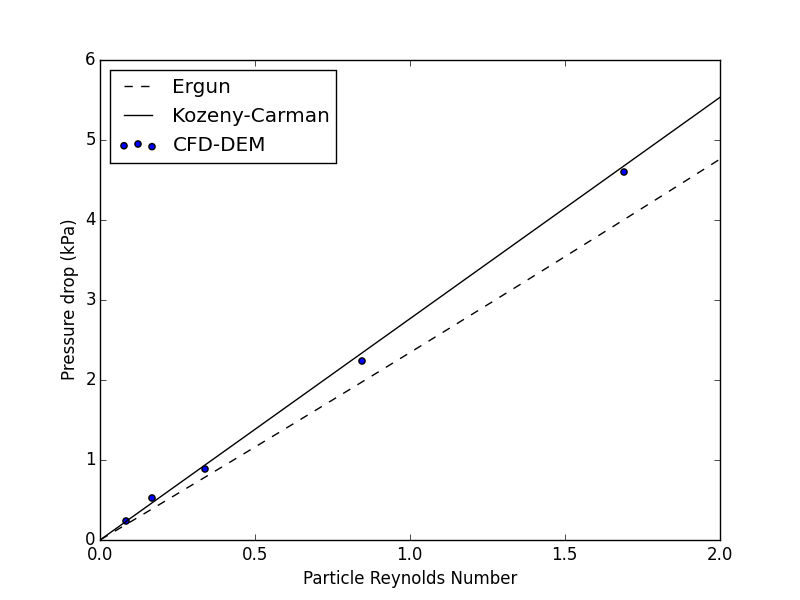
\includegraphics[width=\textwidth]{chapters/figures/pressureDrops-full.png}
                \caption{Well-packed bed}
                \label{fig:pressure-drop-full}
        \end{subfigure}%
        
          %add desired spacing between images, e. g. ~, \quad, \qquad, \hfill etc.
          %(or a blank line to force the subfigure onto a new line)
        \begin{subfigure}[b]{0.75\textwidth}
                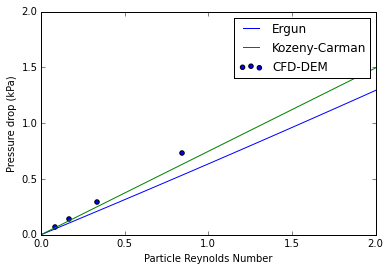
\includegraphics[width=\textwidth]{chapters/figures/pressureDrops-evap.png}
                \caption{Re-settled bed}
                \label{fig:pressure-drop-evap}
        \end{subfigure}
        \caption{Pressure drop calculations across packed beds, solved by CFD-DEM, fit well to the Kozeny-Carman empirical relation.}\label{fig:cfdem-pressure-drop}
\end{figure}



\begin{figure}[t]
	\centering
	\caption{Cut-away view of the pebble bed with streamlines of helium moving in generally straight paths from inlet to exit.}
	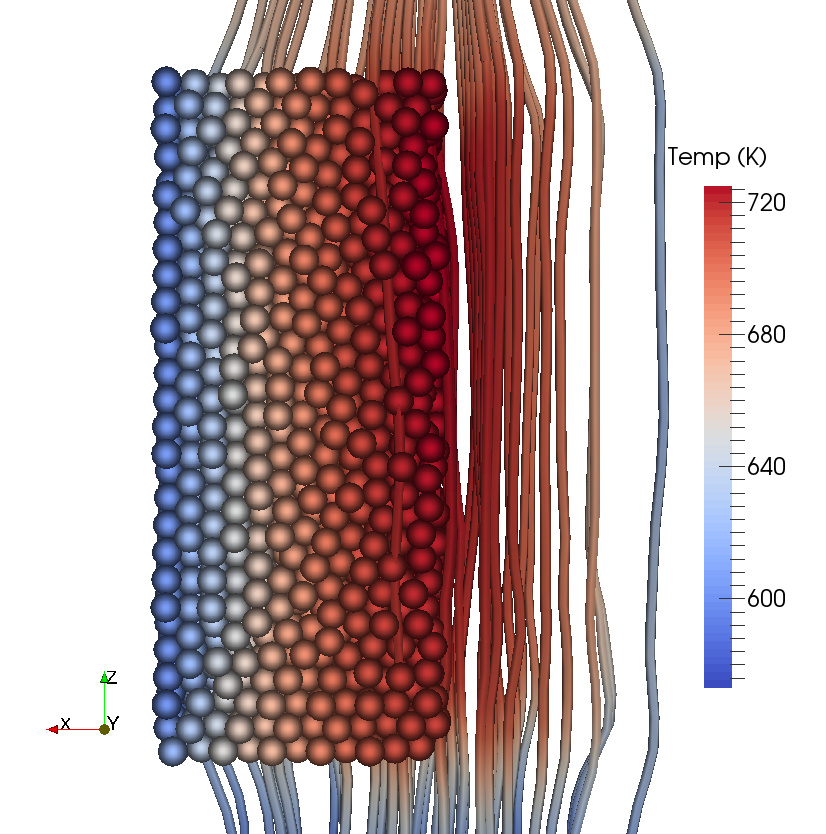
\includegraphics[width=0.75\textwidth]{chapters/figures/cfd-dem-streamlines2}\label{fig:cfdem-streamlines}
\end{figure}




\begin{figure}
        \centering
        \begin{subfigure}[b]{0.75\textwidth}
                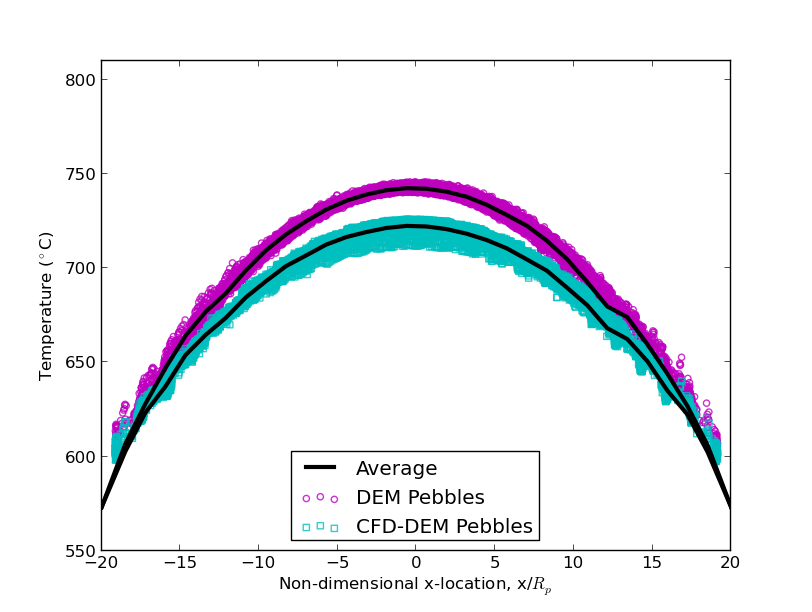
\includegraphics[width=\textwidth]{chapters/figures/full-x-T-color}
                \caption{Well-packed bed}
                \label{fig:x-T-full}
        \end{subfigure}%
        
          %add desired spacing between images, e. g. ~, \quad, \qquad, \hfill etc.
          %(or a blank line to force the subfigure onto a new line)
        \begin{subfigure}[b]{0.75\textwidth}
                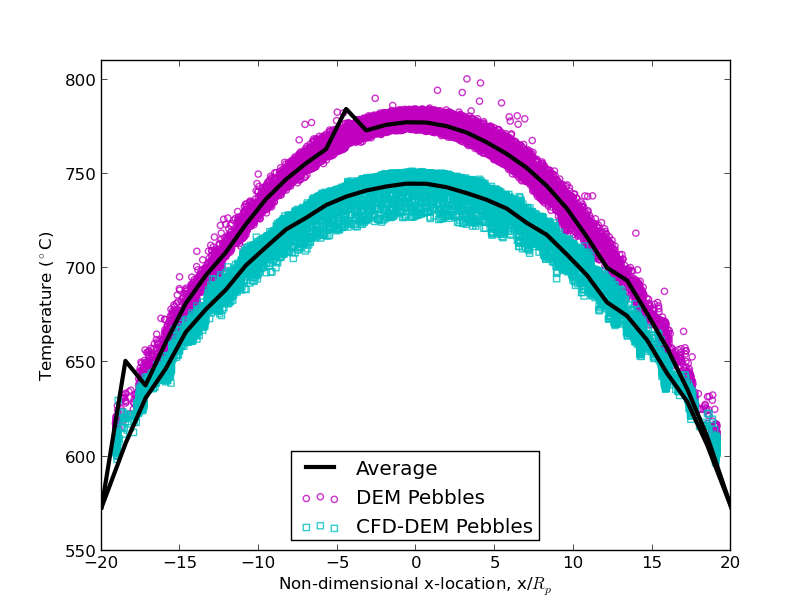
\includegraphics[width=\textwidth]{chapters/figures/evap-x-T-color}
                \caption{Re-settled bed}
                \label{fig:x-T-evap}
        \end{subfigure}
        \caption{Scatter temperature profiles of pebbles in a bed that is: well-packed (left) and resettled after 10\% of pebbles were removed from crushing (right). The introduction of helium into the simulation contributes to both lower overall temperatures (higher effective conductivity) and the smoothing out of high temperatures of isolated pebbles.}\label{fig:cfdem-x-T}
\end{figure}

\subsection{Effective thermal conductivity from CFD-DEM}

The well-packed and resettled pebble beds were run to thermal steady-state with nuclear heating and wall cooling in both pure DEM and coupled CFD-DEM simulations for comparison. From steady-state temperature distributions, seen in the pebble scatter plots in Fig. 3, an average profile is calculated and an effective thermal conductivity computed. The values are tabulated in Table I. 
In the case of pure DEM, energy is transported solely along conduction routes in the ensemble. When the packing of the bed is disturbed, this results in a substantial drop in effective conductivity (a drop of 31\%). The details of the conductivity reduction were studied extensively in Ref. 23. Perhaps more important than the reduction in effective conductivity, is the appearance of isolated pebbles. Because heat deposition is volumetrically applied, pebbles with poor conduction routes become much hotter than their neighbors. This is evident in the high temperatures seen in many of the pebbles in the right figure of Fig. 3. Over-heating of isolated pebbles could induce sintering and impact their tritium release even when the average temperatures measured in the bed are well below sintering values.
When CFD-DEM beds are analyzed, there is still a large reduction in effective conductivity (22\% drop), but interesting to note is the lack of isolated pebbles with high temperatures. In the CFD-DEM scatter plot of the right image in Fig. 3, there is evidence of the reduced heat transfer in the same region as the isolated pebbles from the DEM bed, but the temperatures are much closer to the average values of neighboring pebbles. The helium purge gas has effectively smoothed out the temperatures and provided heat transport paths for any pebbles that have loose physical contact with neighbors.
In spite of the 22\% decrease in effective conductivity, the maximum temperature of the pebble bed only increased 6.2\% (from 725 to 751 K) when helium is included in the model. This result is significant for solid breeder designers. They may choose a solid breeder volume such that in the event of extensive pebble cracking, the maximum temperature of the bed would remain within the ideal windows dictate for the lithium ceramics.

\begin {table}[htp] %
\caption{Pebble bed values from the test matrix of the beds analyzed in this study.}
\label {tab:cfdem-keff} \centering %
\begin {tabular}{ rccccc }
\toprule %
			& 	\multicolumn{2}{c}{$k_\text{eff}$}	&   \multicolumn{2}{c}{$T_\text{max}$}	&	$\frac{Q_h}{Q_\text{nuc}}$		\\
			& 	\multicolumn{2}{c}{(W/mK)}			&	\multicolumn{2}{c}{(K)}				&									\\
			& 	DEM 		& 	CFD-DEM				&	DEM 		& 	CFD-DEM 			& 	CFD-DEM							\\\toprule
Well-packed	& 	0.96		& 	1.09				& 	745			& 	725					& 	1.15							\\
Resettled	& 	0.66		& 	0.85				& 	800			& 	751					& 	1.52							\\\bottomrule
\end{tabular}
\end{table}




An accompanying result is the increased amount of energy carried out of the system by the helium purge gas. In Table I, the last column provides the ratio of energy carried out of the system to the nuclear energy deposited into the bed. The amount of energy carried out by the helium increased from 1.15\% to 1.52\% from ‘well-packed’ to ‘resettled’.
evap-x-T-color
The CFD-DEM formulation maintains calculations of pebble-pebble interactions while dynamically coupling to the helium flow. The model demonstrates the ability of helium gas to smooth out any hot spots predicted by pure-conduction DEM formulations. Further, the lattice-Boltzmann simulation, while not fully coupled to DEM, revealed important features of helium flow in volumetrically heated pebble beds – mainly the smearing of temperature profiles along the paths of cooling.
%%%%%%%%%%%%%%%%%%%%%%%%%%%%%%%%%%%%%%%%%%